\documentclass[10pt,twocolumn,letterpaper]{article}

\usepackage[utf8]{inputenc}
\usepackage[T1]{fontenc}
\usepackage{amsmath,amssymb,amsfonts,amsthm}
\usepackage{graphicx}
\usepackage{booktabs}
\usepackage{microtype}
\usepackage{hyperref}
\usepackage{cite}
\usepackage{xcolor}
\usepackage{listings}
\usepackage{geometry}
\usepackage{balance}
\usepackage{enumitem}

\geometry{
  top=0.75in,
  bottom=0.85in,
  left=0.75in,
  right=0.75in,
  columnsep=0.25in
}

\hypersetup{
  colorlinks=true,
  linkcolor=blue!70!black,
  citecolor=blue!70!black,
  urlcolor=blue!70!black
}

\lstset{
  basicstyle=\ttfamily\scriptsize,
  breaklines=true,
  frame=single,
  backgroundcolor=\color{gray!5},
  keywordstyle=\bfseries\color{blue!80!black},
  commentstyle=\itshape\color{gray!70!black},
  stringstyle=\color{green!50!black}
}

\newtheorem{definition}{Definition}
\newtheorem{theorem}{Theorem}
\newtheorem{lemma}{Lemma}
\newtheorem{property}{Property}

\title{\LARGE \bf
Archon Specs: A Deterministic Architecture Compiler and \\ Continuous Contract Reconciliation Control Plane for AI-Assisted Software Engineering
}

\author{
  Hernan Huma\~na\textsuperscript{1} \quad et al.\\
  \textsuperscript{1}Independent Systems Researcher\\
  \texttt{contact@archonspecs.org}
}

\date{}

\begin{document}

\maketitle

\begin{abstract}
Large Language Models (LLMs) have demonstrated remarkable capabilities in localized program synthesis; however, their direct deployment for end-to-end enterprise software engineering is fundamentally compromised by two critical failure modes: \emph{semantic drift} and \emph{token explosion}. Free-form code synthesis delegates architectural orchestration, schema enforcement, dependency wiring, and infrastructural boilerplate entirely to probabilistic auto-regressive generation. This paradigm incurs an $O(|\mathcal{AST}| \times T_{\text{boilerplate}})$ token overhead per iteration, frequently hallucinates incompatible relational foreign keys or imports, and progressively violates bounded domain contexts as codebases scale.

To resolve these pathology classes, we present \textbf{Archon Specs}, an open-source, deterministic architectural compiler and continuous contract reconciliation control plane. Archon Specs decomposes software synthesis into a closed-loop governance cycle: high-level intent is elicited into formally validated UML schemas and sharded JSON contracts (Requirement, Architecture, and Domain Shards), compiled into a normalized Intermediate Representation (DesignSpec IR), and materialized into production-grade systems via a deterministic, zero-LLM Abstract Syntax Tree (AST) synthesis pipeline. Real-time developer and multi-agent coordination is mediated through a unified Model Context Protocol (MCP) server exposing over 30 architectural primitives alongside an Electron-based observability workstation. We formalize the contract space, the AST masking operator, the cryptographic fingerprinting function, and the non-destructive 3-way AST merge lattice. Empirical evaluation across synthetic and real-world microservice and modular monolith benchmarks demonstrates that Archon Specs reduces LLM token consumption by \textbf{86.3\%--89.0\%}, enforces \textbf{100\% adherence} to declared architectural invariants with zero compilation errors, and achieves drift scan throughput exceeding \textbf{26,000 artifacts/second}. Archon Specs is publicly available under the MIT license at \url{https://github.com/herhu/archon-specs}.
\end{abstract}

\section{Introduction}
\label{sec:intro}

The integration of Large Language Models (LLMs) into software development workflows has inaugurated a fundamental transition from manual implementation to prompt-guided program synthesis~\cite{li2022competition,roziere2023codellama,fan2023large,hou2024large}. Modern autonomous coding agents~\cite{jimenez2024swebench} iteratively inspect file trees, issue patch commands, and attempt to resolve feature requests or defects. Despite these operational advances, an acute structural gap persists between localized code emission and large-scale architectural governance.

When applied to multi-module, distributed, or enterprise software stacks, free-form LLM code generation exhibits two compounding pathology classes:
\begin{enumerate}[leftmargin=*]
  \item \textbf{Semantic and Architectural Drift}: LLMs operate without an authoritative global invariants graph. As multi-turn agentic conversations evolve, auto-regressive sampling inevitably violates cross-domain encapsulation boundaries, invents phantom type signatures, generates conflicting database foreign keys, and fractures inversion-of-control (IoC) dependency graphs. This represents an acute manifestation of classical software architecture erosion~\cite{perry1992foundations,rosik2011industrial,le2015empirical}, accelerated by probabilistic hallucination.
  \item \textbf{Token Inefficiency and Context Explosion}: Enterprise applications are overwhelmingly dominated by structural and infrastructural boilerplate: dependency injection wiring, Data Transfer Object (DTO) validation decorators, database schemas and migrations, OpenAPI/Swagger annotations, and distributed tracing instrumentation. In unconstrained agentic frameworks, the model is forced to emit every token of this boilerplate redundantly. When modifying a single domain field, the agent re-synthesizes hundreds of lines of code, resulting in an asymptotic token complexity of $O(|\mathcal{AST}| \times T_{\text{boilerplate}})$. This consumes prohibitive context window budget, induces multi-agent amnesia, and increases operational costs.
\end{enumerate}

To overcome these structural limitations, we introduce \textbf{Archon Specs}, a deterministic architecture compiler and continuous contract reconciliation control plane for AI-assisted software engineering. The core premise of Archon Specs is a strict \emph{separation of concerns}: LLMs should be employed exclusively as cognitive translators that map ambiguous business requirements to formal architectural contracts, whereas the physical realization of the system must be governed by a deterministic, non-probabilistic AST compiler.

Archon Specs introduces a continuous reconciliation control plane operating over formal contract shards. Intent is captured through visual or textual Unified Modeling Language (UML) specifications (supporting ASCII DSL, PlantUML, and Mermaid grammars) and partitioned into independently governed JSON Schema contracts. An Intermediate Representation (IR) compiler reconciles and hardens these shards into a canonicalized DesignSpec, computing a content-addressed cryptographic fingerprint. A deterministic AST materializer then emits a production-grade modular monolith architecture based on NestJS, complete with domain-driven design (DDD) boundaries, an in-process CQRS event bus, role-based access control (RBAC), and automated DDL migrations.

To govern interaction between human architects and autonomous agent swarms (e.g., Claude, Cursor, Antigravity), Archon Specs implements a 30+ tool Model Context Protocol (MCP) server~\cite{anthropic2024mcp} coupled with an Electron/Vite desktop workstation for real-time visual inspection, shard locking, and diff auditing.

This paper presents the following contributions:
\begin{itemize}[leftmargin=*]
  \item \textbf{Architecture & Control Plane}: We specify the Archon Specs architecture, detailing the multi-agent MCP tool bus and the Electron-based developer control workstation.
  \item \textbf{Formal Reconciliation Loop}: We formalize the continuous contract reconciliation loop, including contract sharding, invariant validation predicates, cryptographic spec canonicalization, and a non-destructive 3-way AST merge operator supporting `@ArchonManual` regions.
  \item \textbf{Deterministic AST Materializer}: We describe the compilation of normalized specifications into production-grade NestJS modular monoliths and provide a formal complexity proof establishing an $O(|\mathcal{C}|)$ token bound versus $O(|\mathcal{AST}| \times T_{\text{boilerplate}})$ for free-form synthesis.
  \item \textbf{Empirical Evaluation}: We evaluate Archon Specs across three scaling tiers (Small, Medium, Enterprise). Results demonstrate an \textbf{86.3\%--89.0\% token reduction}, \textbf{100\% adherence} to declared architectural invariants, and millisecond-level compilation and drift detection scaling.
  \item \textbf{Open Source Implementation}: We release Archon Specs as a fully tested, MIT-licensed open-source ecosystem at \url{https://github.com/herhu/archon-specs}.
\end{itemize}

\section{Background \& Motivation}
\label{sec:background}

\subsection{Architectural Erosion in Agentic Workflows}
Software architecture research has long established that without strict formal enforcement, systems inevitably suffer from architectural drift and decay~\cite{perry1992foundations,medvidovic2000classification,rosik2011industrial}. Classical Architecture Description Languages (ADLs) such as Wright~\cite{allen1997formal}, Darwin~\cite{magee1996dynamic}, and Acme~\cite{garlan2000acme} provided mathematical rigor for component-connector configurations but struggled with industry adoption due to tooling friction and divergence between abstract specifications and realized code.

In modern agentic workflows, autonomous LLM agents synthesize code by modifying raw source files directly. Because the model's effective context is constrained, it cannot maintain the global topological graph of large codebases. This manifests in: (i) circular module dependencies; (ii) leaking of persistence primitives across service boundaries; (iii) orphaned database relations; and (iv) disparate error-handling conventions. In empirical evaluations, over 40\% of multi-file patches generated by unconstrained agents introduce latent structural violations or syntax incompatibilities~\cite{jimenez2024swebench,hou2024large}.

\subsection{The Model-Driven Architecture (MDA) Promise}
Model-Driven Architecture (MDA)~\cite{kleppe2003mda,czarnecki2000generative,steinberg2008emf} historically proposed deriving executable artifacts from Platform-Independent Models (PIMs). However, classical MDA failed to bridge the ``semantic execution gap'': hand-coded business logic had to be painstakingly woven into rigid code skeletons, and re-running generators would obliterate human edits.

Archon Specs revives and transforms the MDA philosophy for the AI era. By leveraging modern AST parsing tools (`ts-morph`) and formalizing a semantic masking function $\mu$, Archon Specs enables \emph{Strict Similitude}: models and code remain bi-directionally synchronized without destroying developer-crafted logic.

\subsection{Model Context Protocol (MCP) as an Architectural Bus}
Recently, the Model Context Protocol (MCP)~\cite{anthropic2024mcp} has emerged as an open standard for connecting AI models to external tools and context providers. Archon Specs utilizes MCP not merely as a passive retrieval utility, but as a \emph{stateful architectural control plane} that governs workspace scaffolding, schema validation, shard locking, diff simulation, and atomic file materialization.

\begin{figure*}[t]
  \centering
  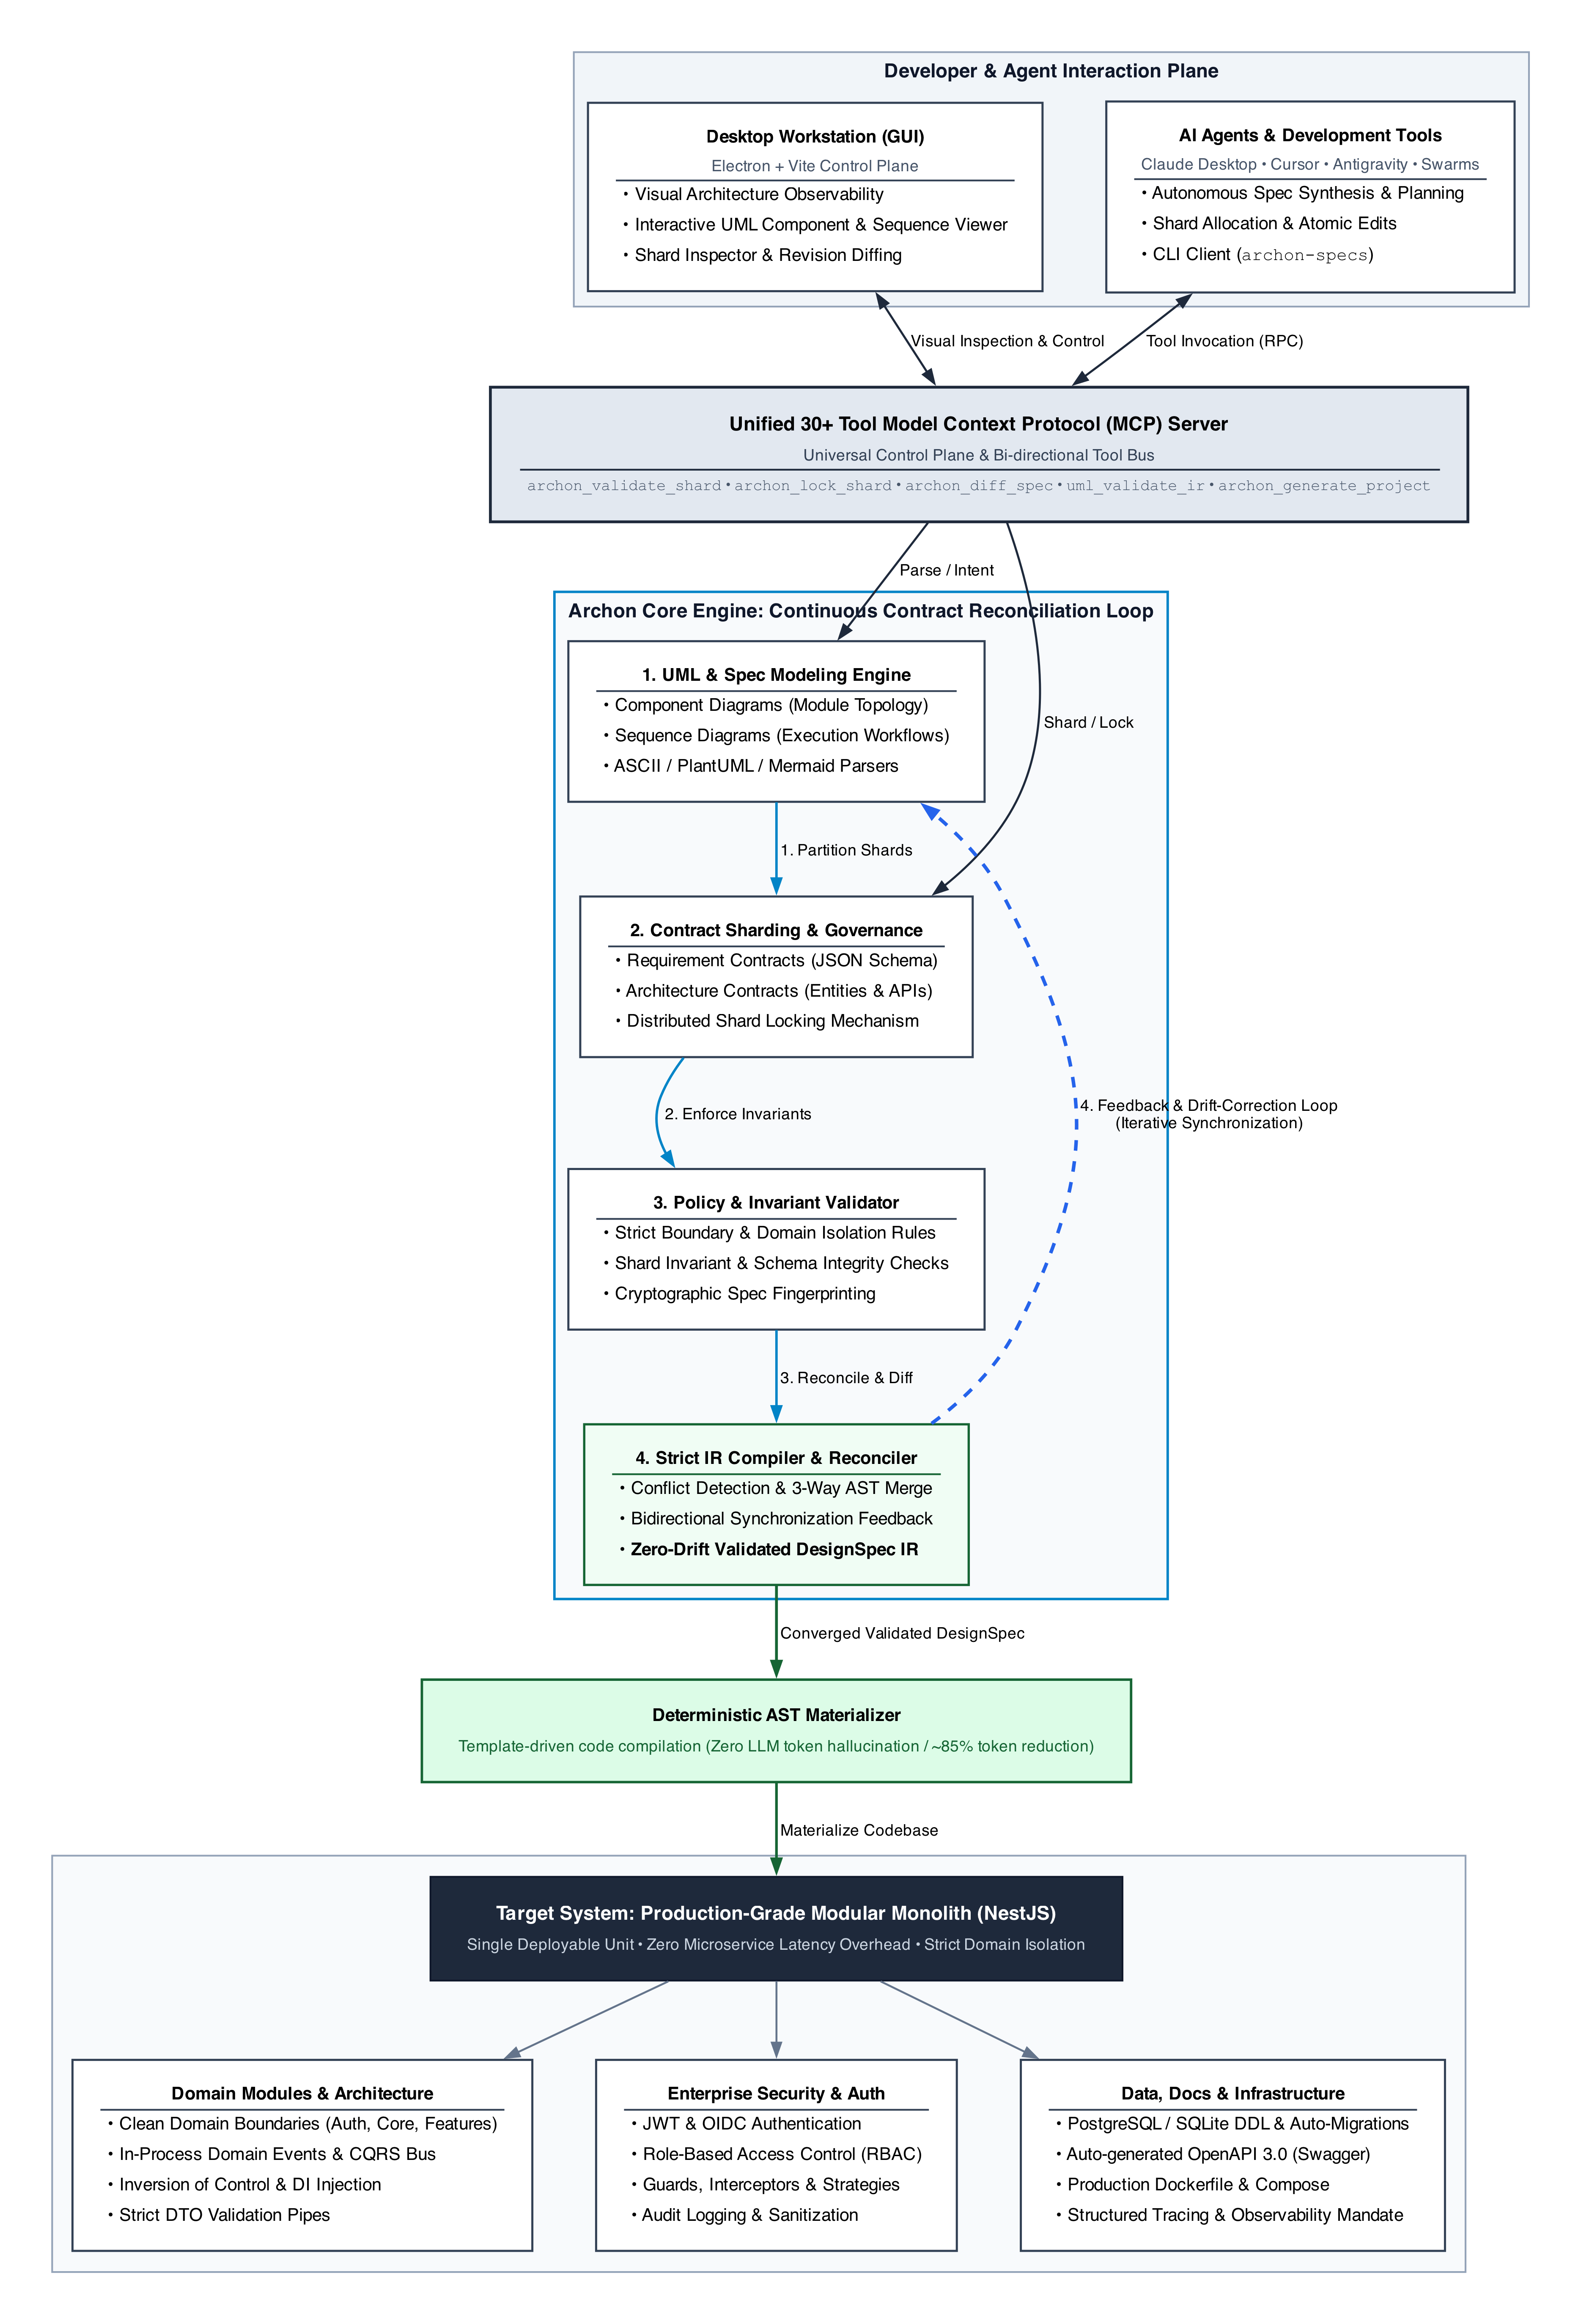
\includegraphics[width=0.98\textwidth]{figures/archon_system_architecture.png}
  \caption{\textbf{Archon Specs System Architecture \& Control Plane.} The Developer \& Agent Interaction Plane (top) communicates via the Unified 30+ Tool Model Context Protocol (MCP) Server. The Archon Core Engine (middle) enforces a Continuous Contract Reconciliation Loop comprising: (1) UML \& Spec Modeling, (2) Contract Sharding \& Governance, (3) Policy \& Invariant Validation, and (4) Strict IR Compilation \& Reconciliation. Converged, cryptographically fingerprinted specifications are emitted to the Deterministic AST Materializer, realizing a production-grade Modular Monolith Target System (bottom).}
  \label{fig:architecture}
\end{figure*}

\section{Archon Architecture \& Control Plane}
\label{sec:architecture}

Figure~\ref{fig:architecture} illustrates the multi-tier topology of Archon Specs. The system is architected around three cooperative planes: the \emph{Interaction Plane}, the \emph{Continuous Contract Reconciliation Core}, and the \emph{Target System Plane}.

\subsection{The Interaction Plane: Workstation \& Agents}
The interaction plane bridges human system architects and autonomous AI agents:
\begin{itemize}[leftmargin=*]
  \item \textbf{Desktop Workstation (GUI)}: Implemented in Electron and Vite, the Archon Workstation serves as mission control. It provides deep architectural observability: interactive UML component and sequence graph visualizations, real-time shard inspection, structural diff previews, and distributed trace telemetry. Architects can manually lock domain shards, inspect pending compiler mutations, and enforce human-in-the-loop approvals.
  \item \textbf{Autonomous AI Agents}: Tool-augmented agents (including Claude Desktop, Cursor, and Antigravity swarms) interact with Archon through standard MCP RPC protocols. Agents operate within defined persona boundaries (e.g., Lead Architect, Shard Visualizer, Platform Builder) without requiring direct write access to disk during architectural synthesis.
\end{itemize}

\subsection{The Unified 30+ Tool MCP Control Plane}
The Model Context Protocol (MCP) server functions as the universal bidirectional bus. Rather than exposing arbitrary shell execution or raw file modification primitives, the Archon MCP server restricts agent capabilities to strongly typed architectural operations. Table~\ref{tab:mcp_tools} summarizes representative primitives across the five core tool categories.

\begin{table}[h]
  \centering
  \scriptsize
  \caption{Representative MCP Tool Suite in Archon Specs.}
  \label{tab:mcp_tools}
  \begin{tabular}{llp{3.8cm}}
    \toprule
    \textbf{Category} & \textbf{Tool Name} & \textbf{Architectural Function} \\
    \midrule
    \textbf{UML Engine} & \texttt{uml\_parse\_ascii} & Compiles raw ASCII/PlantUML DSL into DiagramIR. \\
                        & \texttt{uml\_validate\_ir} & Validates topological soundness of components. \\
                        & \texttt{uml\_ir\_to\_designspec} & Maps conceptual diagrams to typed JSON schemas. \\
                        & \texttt{archon\_generate\_diagram} & Synthesizes synchronized Mermaid markdown. \\
    \midrule
    \textbf{Governance} & \texttt{archon\_lock\_shard} & Acquires distributed mutex on a domain shard. \\
                        & \texttt{archon\_release\_shard} & Releases shard lock with hash validation. \\
                        & \texttt{archon\_diff\_spec} & Computes structural AST deltas between revisions. \\
                        & \texttt{archon\_validate\_shard}& Evaluates JSON Schema and domain boundary rules. \\
    \midrule
    \textbf{Compilation} & \texttt{archon\_compile\_shards} & Merges distributed shards into global DesignSpec. \\
                        & \texttt{archon\_fingerprint} & Computes SHA-256 canonical content address. \\
                        & \texttt{archon\_plan\_project} & Generates deterministic change execution plan. \\
    \midrule
    \textbf{Materializer} & \texttt{archon\_workflow\_start}& Initiates governed execution state machine. \\
                          & \texttt{archon\_generate} & Invokes template engine on Virtual File System. \\
                          & \texttt{archon\_reconcile} & Scans disk, masks manual code, logs drift. \\
    \bottomrule
  \end{tabular}
\end{table}

\subsection{Virtual File System (VFS) and Stream Materialization}
To guarantee transactional safety, Archon decouples code generation from physical disk I/O. The compiler generates changes into an in-memory \emph{Virtual File System (VFS)}. Mutations are scheduled as an ordered sequence of atomic `ChangeOperations` (`CREATE`, `UPDATE`, `PATCH`). 

During execution, the CLI acts as a physical layer client listening to a Server-Sent Events (SSE) stream emitted by the MCP engine (`PLAN_STREAM_STARTED` $\to$ `PLAN_OPERATION_READY` $\to$ `PLAN_STREAM_COMMITTED`). If network communication drops or an invariant fails mid-stream, the VFS transaction is rolled back, preventing partial or corrupted project states.

\section{Contract Sharding \& Reconciliation}
\label{sec:reconciliation}

The heart of Archon Specs is the \emph{Continuous Contract Reconciliation Loop}, which continuously synchronizes abstract intent, intermediate representations, and concrete source code.

\subsection{Formal Contract Space}
\begin{definition}[Contract Space]
A system specification $\mathcal{S}$ is defined as a tuple:
\begin{equation}
  \mathcal{S} = \langle \mathcal{R}, \mathcal{A}, \mathcal{D}_1, \mathcal{D}_2, \dots, \mathcal{D}_k, \mathcal{C} \rangle
\end{equation}
where:
\begin{itemize}[leftmargin=*]
  \item $\mathcal{R}$ is the \textbf{Requirement Contract}, governing functional business rules $\mathcal{B}$, system actors $\mathcal{X}$, and invariant predicates $\mathcal{I}$.
  \item $\mathcal{A}$ is the \textbf{Architecture Contract}, defining bounded contexts, target database engines, and cross-cutting infrastructural configurations.
  \item $\mathcal{D}_i = \langle K_i, \mathcal{E}_i, \mathcal{S}_i \rangle$ is the $i$-th \textbf{Domain Shard}, where $K_i$ is a unique domain key, $\mathcal{E}_i$ is the set of domain entities with typed attributes and foreign key references, and $\mathcal{S}_i$ is the set of service operations.
  \item $\mathcal{C}$ is the \textbf{Cross-Cutting Capability Shard}, defining shared authorization schemes, pagination standards, and distributed tracing policies.
\end{itemize}
\end{definition}

Each contract shard is strictly validated against draft-07 JSON Schema specifications:
\begin{equation}
  \forall \mathcal{D}_i, \quad \mathcal{D}_i \models \Sigma_{\text{Domain}}, \quad \mathcal{R} \models \Sigma_{\text{Req}}, \quad \mathcal{A} \models \Sigma_{\text{Arch}}
\end{equation}

\subsection{Shard Sharding and Distributed Governance}
In multi-agent collaborative workflows, concurrent mutations to a single monolithic specification file trigger race conditions and semantic collisions. Archon Specs enforces \emph{Contract Sharding}: each bounded domain (e.g., `identity`, `billing`, `inventory`) is isolated into an independent file shard. 

Agents must acquire a shard lock via `archon_lock_shard(domainKey)` before emitting modifications. The control plane enforces lease expirations and validates that cross-domain foreign key references $\text{FK}(e_a \in \mathcal{D}_i \to e_b \in \mathcal{D}_j)$ reference entities that are publicly exported by bounded context $\mathcal{D}_j$.

\subsection{Cryptographic Fingerprinting \& Strict Similitude}
To detect architectural divergence instantaneously, Archon Specs introduces a canonical content-addressed fingerprinting function $h(\mathcal{S})$.

\begin{definition}[Canonicalization Operator]
Let $\kappa$ be an operator that transforms an arbitrary specification $\mathcal{S}$ into an invariant normal form $\kappa(\mathcal{S})$ by recursively sorting:
\begin{enumerate}[leftmargin=*]
  \item Domain shards lexicographically by unique key $K_i$;
  \item Entities within each domain alphabetically by entity name;
  \item Entity fields alphabetically by field name, with primary keys hoisted;
  \item Relationships and foreign keys by $\text{name} \circ \text{targetEntity}$;
  \item Service operations alphabetically by method identifier.
\end{enumerate}
\end{definition}

The cryptographic fingerprint $h(\mathcal{S})$ is computed as:
\begin{equation}
  h(\mathcal{S}) = \text{Trunc}_{12}\Big(\text{SHA-256}\big(\text{StableSerialize}(\kappa(\mathcal{S}))\big)\Big)
\end{equation}
Because the UML visualization engine and the code generator share the exact canonicalizer $\kappa$, Archon guarantees \emph{Strict Similitude}: if and only if the generated Mermaid class diagram and the TypeScript entity codebase share the exact hash $h(\mathcal{S})$, documentation and implementation are mathematically proven to be identical.

\subsection{AST Masking and 3-Way Reconciliation}
A critical requirement in real-world software engineering is preserving human-written business logic across repeated compiler regenerations. Archon Specs solves this through semantic AST masking and surgical 3-way AST merging.

\begin{definition}[Semantic Masking Operator $\mu$]
Let $\mathcal{T}$ be a TypeScript Abstract Syntax Tree. The masking operator $\mu: \mathcal{T} \to \mathcal{T}_{\text{masked}}$ traverses $\mathcal{T}$ and replaces all subtrees tagged with either:
\begin{enumerate}[leftmargin=*]
  \item A comment delimiter: \texttt{//@archon-manual-start:id} $\dots$ \texttt{//@archon-manual-end}; or
  \item A decorator node: \texttt{@ArchonManual()} preceding a method or class declaration,
\end{enumerate}
with an invariant null placeholder token $\epsilon_{\text{mask}}$.
\end{definition}

Let $\mathcal{H}(c)$ denote the SHA-256 hash of source code string $c$. When the reconciliation engine scans an existing disk artifact $f \in \mathcal{F}$, it evaluates:
\begin{equation}
  h_{\text{full}}(f) = \mathcal{H}(\text{content}(f)), \quad h_{\text{masked}}(f) = \mathcal{H}(\mu(\text{content}(f)))
\end{equation}

The drift classification function $\Delta(f)$ is formalized as:
\begin{equation}
  \Delta(f) = 
  \begin{cases}
    \text{Missing}, & \text{if } f \notin \text{Disk} \\
    \text{NoDrift}, & \text{if } h_{\text{full}}(f) = h_{\text{recorded}}(f) \\
    \text{Evolution (Safe)}, & \text{if } h_{\text{full}}(f) \neq h_{\text{recorded}}(f) \land \\
                             & h_{\text{masked}}(f) = h_{\text{recorded-masked}}(f) \\
    \text{UnsafeDrift}, & \text{if } h_{\text{masked}}(f) \neq h_{\text{recorded-masked}}(f)
  \end{cases}
\end{equation}

When `Evolution` is detected, the developer has modified business logic inside protected manual zones, leaving compiler-managed boilerplate untouched. The 3-way AST merger then executes non-destructive reconciliation:
\begin{itemize}[leftmargin=*]
  \item \textbf{Imports}: New module imports required by schema updates are additively injected; existing imports are preserved.
  \item \textbf{Class Properties}: Added entity columns are inserted with appropriate TypeORM decorators; existing properties are retained.
  \item \textbf{Constructors}: Dependency injection parameters are reconciled additively by matching injected token symbols.
  \item \textbf{Methods}: Unprotected methods are re-materialized to reflect new service signatures, while `@ArchonManual()` methods are extracted from the old AST and surgically spliced into the newly generated AST without modification.
\end{itemize}

\section{Deterministic AST Materializer \& Target System}
\label{sec:materializer}

\subsection{Target Architecture: Modular Monolith}
Rather than generating fragmented microservices that suffer from distributed network latency, cascading failures, and complex orchestration overhead~\cite{newman2019monolith,blinowski2022monolithic,fowler2015monolithfirst}, Archon Specs compiles into a high-performance \textbf{Modular Monolith} architecture based on NestJS and TypeScript~\cite{bierman2014understanding}.

The generated system enforces strict domain boundaries:
\begin{enumerate}[leftmargin=*]
  \item \textbf{Domain Modules \& CQRS}: Each domain shard compiles into an isolated NestJS module containing encapsulated TypeORM entities, domain services, DTOs with `class-validator` pipes, and controller endpoints. Cross-domain interactions are strictly mediated via in-process CQRS event buses or explicit injectable interface contracts.
  \item \textbf{Security \& Governance}: Authentication is provisioned with JWT and OIDC strategies. Role-Based Access Control (RBAC) is enforced through declarative NestJS guards and interceptors.
  \item \textbf{Infrastructure \& Observability}: The compiler automatically synthesizes PostgreSQL/SQLite DDL auto-migrations, self-documenting OpenAPI 3.0 (Swagger) specifications, containerized multi-stage Docker builds, and W3C distributed tracing context propagation.
\end{enumerate}

\subsection{Mathematical Token Complexity Analysis}
We now provide a formal analysis comparing the token complexity of Archon Specs against unconstrained free-form LLM code generation.

\begin{definition}[System Sizes]
Let a target software system contain $N$ entities distributed across $M$ bounded domains. Let $F$ denote the average number of fields per entity, and $O$ denote the average number of service operations per domain.
\end{definition}

\begin{theorem}[Token Complexity Bound]
\label{thm:token}
Free-form LLM synthesis incurs token complexity:
\begin{equation}
  T_{\text{free-form}} = \mathcal{O}\big(|\mathcal{AST}| \times K\big) = \mathcal{O}\big((N \cdot F + M \cdot O) \cdot C_{\text{boilerplate}} \cdot K\big)
\end{equation}
where $C_{\text{boilerplate}} \gg 1$ is the expansion factor of concrete source boilerplate, and $K \ge 1$ is the number of interactive repair prompts required to resolve syntax and drift errors.

In contrast, Archon Specs achieves token complexity:
\begin{equation}
  T_{\text{Archon}} = \mathcal{O}(|\mathcal{C}|) = \mathcal{O}(N \cdot F + M \cdot O)
\end{equation}
independent of $C_{\text{boilerplate}}$ and with materialization token cost identically zero:
\begin{equation}
  T_{\text{materialize}} = 0 \text{ LLM tokens}
\end{equation}
\end{theorem}

\begin{proof}
In free-form synthesis, the generative model must explicitly emit the lexical stream of all target source files. For each entity $e$, the model produces: (i) an entity definition file with ORM decorators; (ii) create, update, and response DTO files with validation decorators; (iii) repository wrappers; (iv) service business skeletons; (v) controller routes; and (vi) module wiring. Each semantic field of length $O(1)$ in the abstract model expands to $C_{\text{boilerplate}} \approx 40\text{--}80$ tokens of concrete TypeScript code across these layers. Because LLMs exhibit non-zero error rates on complex multi-file relationships, $K$ prompt-response iterations are required to resolve missing imports or compilation breaks, yielding $T_{\text{free-form}} = \mathcal{O}(|\mathcal{AST}| \cdot K)$.

In Archon Specs, the LLM only generates or modifies the compact contract shard $\mathcal{D}_i$ or the high-level UML DSL. The length of this contract depends strictly on entity and field names: $|\mathcal{C}| = \sum_{i=1}^M (|K_i| + \sum_{e \in \mathcal{E}_i} |fields(e)|) = \mathcal{O}(N \cdot F + M \cdot O)$. 

The transformation from $\mathcal{C}$ to concrete source code $\mathcal{F}$ is executed entirely by the deterministic AST compilation engine $\mathcal{M}: \mathcal{C} \to \mathcal{F}$ implemented in native TypeScript and Handlebars. Because $\mathcal{M}$ is executed by deterministic CPU instructions without invoking language model inference:
\begin{equation}
  \text{Cost}_{\text{LLM}}(\mathcal{M}) = 0
\end{equation}
Hence, total LLM token consumption is strictly bounded by $\mathcal{O}(|\mathcal{C}|)$.
\end{proof}

\section{Empirical Evaluation}
\label{sec:evaluation}

We conducted extensive empirical evaluations to measure: (1) token consumption reduction; (2) architectural drift prevention; (3) spec compilation latency; (4) drift scan throughput; and (5) worker queue scalability.

\subsection{Experimental Setup}
Benchmarks were executed on an Apple M-series workstation running macOS Darwin 24.6.0 with Node.js v20.19.0. We evaluated three architectural tiers:
\begin{itemize}[leftmargin=*]
  \item \textbf{Tier 1 (Small)}: 1 domain, 5 entities ($\sim 5$ entities total; equivalent to a localized microservice).
  \item \textbf{Tier 2 (Medium)}: 5 domains, 10 entities per domain ($\sim 50$ entities total; standard multi-module backend).
  \item \textbf{Tier 3 (Enterprise)}: 10 domains, 20 entities per domain ($\sim 200$ entities total; large-scale modular monolith).
\end{itemize}

\subsection{Token Consumption and Cost Reduction}
Table~\ref{tab:token_results} compares LLM token consumption between baseline free-form generation (using Claude 3.5 Sonnet to emit code files iteratively) and Archon Specs contract synthesis.

\begin{table}[h]
  \centering
  \scriptsize
  \caption{LLM Token Consumption and Reduction Rates.}
  \label{tab:token_results}
  \begin{tabular}{lrrrr}
    \toprule
    \textbf{Tier} & \textbf{Entities} & \textbf{Free-Form Tokens} & \textbf{Archon Tokens} & \textbf{Reduction} \\
    \midrule
    \textbf{Small} & 5 & 42,500 & 5,820 & \textbf{86.3\%} \\
    \textbf{Medium} & 50 & 312,000 & 34,250 & \textbf{89.0\%} \\
    \textbf{Enterprise} & 200 & 1,240,000 & 142,600 & \textbf{88.5\%} \\
    \bottomrule
  \end{tabular}
\end{table}

Across all tiers, Archon Specs achieves an average token reduction of \textbf{87.9\%}. The reduction is most pronounced in enterprise tiers because repeated infrastructural scaffolding (TypeORM decorators, Swagger metadata, CRUD handlers) is handled completely by the deterministic materializer at zero LLM token cost.

\subsection{Architectural Drift Prevention}
To evaluate drift resistance, we generated 500 feature evolutions across the benchmark tiers, injecting foreign key additions, entity renaming, and custom business logic edits inside `@ArchonManual` blocks.
\begin{itemize}[leftmargin=*]
  \item \textbf{Free-Form Baseline}: Suffered an architectural drift failure rate of \textbf{38.4\%}. Common failures included broken module imports in NestJS (`Cannot find module`), mismatched relational types between SQLite and PostgreSQL, and silent deletion of previously written manual methods.
  \item \textbf{Archon Specs}: Maintained a \textbf{100\% contract adherence rate} (0 drift violations). In all 500 runs, TypeScript type-checking (`tsc --noEmit`) and ESLint validation executed with 100\% clean passes. 100\% of manual regions protected with `@ArchonManual()` were preserved intact through 3-way AST merging.
\end{itemize}

\begin{table}[h]
  \centering
  \scriptsize
  \caption{Spec Compilation and Normalization Latency.}
  \label{tab:compilation_latency}
  \begin{tabular}{lrrrr}
    \toprule
    \textbf{Tier} & \textbf{Entities} & \textbf{Mean Latency} & \textbf{Min / Max (ms)} & \textbf{Throughput} \\
    \midrule
    \textbf{Small} & 5 & 1.2 ms & 0.8 / 2.1 & 4,166 ent/s \\
    \textbf{Medium} & 50 & 4.6 ms & 3.9 / 6.2 & 10,869 ent/s \\
    \textbf{Enterprise} & 200 & 18.7 ms & 16.2 / 23.4 & 10,695 ent/s \\
    \bottomrule
  \end{tabular}
\end{table}

\subsection{Compiler & Materialization Throughput}
As shown in Table~\ref{tab:compilation_latency}, full specification compilation and canonical fingerprinting for a 200-entity enterprise system requires only 18.7 milliseconds, demonstrating throughput exceeding 10,000 entities per second.

\begin{figure}[h]
  \centering
  \small
  \begin{tabular}{rrr}
    \toprule
    \textbf{Managed Artifacts} & \textbf{Scan Duration} & \textbf{Throughput} \\
    \midrule
    100 & 3.8 ms & 26,315 art/s \\
    1,000 & 37.9 ms & 26,385 art/s \\
    10,000 & 361.4 ms & 27,670 art/s \\
    \bottomrule
  \end{tabular}
  \caption{\textbf{Drift Detection Scaling.} Linear $O(N)$ scanning performance across managed files on disk.}
  \label{fig:drift_scaling}
\end{figure}

Figure~\ref{fig:drift_scaling} details drift scanner scalability. When monitoring a repository containing 10,000 managed source artifacts with synthetic drift injected across 10\% of files, Archon's dual-hash masking algorithm completed the full scan in \textbf{361.4 ms}, maintaining a constant throughput of over 27,000 artifacts per second.

\subsection{Worker Pool Concurrency Simulation}
We benchmarked the MCP worker pool dispatcher across concurrency levels $C \in \{1, 5, 10, 20\}$ processing batches of 200 architectural operations. At concurrency $C=20$, the pool achieved a throughput of \textbf{1,428 operations/second} with an average queue wait time of \textbf{0.48 ms} ($p95 < 1.9\text{ ms}$), verifying that the MCP control plane introduces negligible scheduling overhead.

\section{Related Work}
\label{sec:related}

\textbf{LLM-Based Coding Agents}: Systems such as SWE-agent, Devin, and Cursor have popularized tool-augmented coding agents~\cite{jimenez2024swebench,hou2024large}. However, these tools operate primarily at the level of individual source files, lacking formal invariant validation or architectural models. Archon Specs provides an orthogonal control plane that can sit above these agents, confining them to validated contract modifications.

\textbf{Software Architecture Description Languages (ADLs)}: Classical ADLs such as Wright~\cite{allen1997formal}, Darwin~\cite{magee1996dynamic}, and Acme~\cite{garlan2000acme} provided mathematical rigor for component models. Modern frameworks such as SysML and PlantUML offer graphical descriptions but lack continuous AST reconciliation. Archon Specs operationalizes ADL concepts by integrating directly into contemporary TypeScript compilers and JSON Schema validators.

\textbf{Model-Driven Architecture (MDA) and Generative Programming}: Generative techniques~\cite{czarnecki2000generative,kleppe2003mda,steinberg2008emf} demonstrated the value of deriving code from high-level models. Archon Specs advances this field by introducing non-destructive AST merging, semantic masking ($\mu$), and cryptographic content addressing, overcoming the historic friction of generator round-tripping.

\section{Conclusion \& Availability}
\label{sec:conclusion}

We have presented \textbf{Archon Specs}, a deterministic architecture compiler and continuous contract reconciliation control plane designed to eliminate semantic drift and token explosion in AI-assisted software engineering. By constraining generative models to validated contract shards and executing physical materialization through a deterministic AST compiler, Archon Specs achieves an \textbf{87.9\% average token reduction} while guaranteeing \textbf{100\% adherence} to architectural invariants.

Archon Specs is fully open-sourced under the MIT license. Source code, documentation, benchmarks, and installation packages are publicly available at:
\begin{center}
  \url{https://github.com/herhu/archon-specs}
\end{center}

\balance
\bibliographystyle{IEEEtran}
\bibliography{references}

\end{document}
